%%%----------SETUP----------%%%

\documentclass[11pt, titlepage]{article}
\usepackage{lmodern}
\usepackage[margin=1.25in, headheight=14pt]{geometry}
\usepackage{setspace}
    \onehalfspacing
\usepackage[dvipsnames]{xcolor}
\usepackage{tabularray}
\usepackage{nameref}
\usepackage{fancyhdr}
\usepackage[style=apa, natbib=true]{biblatex}
    \addbibresource{left_right.bib}
\usepackage[colorlinks=true, 
            allcolors=RoyalBlue,
            citecolor=.]{hyperref} 
\usepackage{graphicx}
    \graphicspath{ {images/} }
\usepackage{booktabs} 
\usepackage{amsmath}
\usepackage{amssymb}
\usepackage{amsfonts}

\usepackage[english]{babel}
\usepackage[autostyle, english = american]{csquotes}
\MakeOuterQuote{"}
\usepackage{subcaption}
\usepackage{float}

%%  Set biographic information for the title page and document

\newcommand{\thesistitle}{Probing Political Ideology in Large Language Models: How Latent Political Representations Generalize Across Task and Modality}
\newcommand{\thesisauthor}{Tianyi Zhang}
\newcommand{\graddate}{Spring 2026}
\newcommand{\facultyadvisor}{Aaron Schein}
\newcommand{\preceptor}{David Peterson}
\newcommand{\keywords}{Computational Social Science; Political Ideology; Large Language Models; Vision-Language Models; Mechanistic Interpretability; Inference-Time Intervention}

%% Set PDF metadata
\hypersetup{
  pdfauthor={\thesisauthor \ Copyright \textcopyright \number\year},
  pdftitle={\thesistitle},
  pdfsubject={MACSS MA Thesis},
  pdfkeywords={\keywords},
  pdfborder={0 0 0}
}

%% set up header footer style
\pagestyle{fancy}
\fancyhead{}
\fancyhead[R]{\thesisauthor}
\fancyfoot{}
\fancyfoot[C]{\thepage}


\begin{document}

\begin{titlepage}
    %% Do not edit the titlepage section. Make any changes above
    \begin{center}
        \vspace*{-0.45in}
        
\includegraphics[height = 1.5in]{images/Shield.png}\\
	\vspace{0.1in}
        \Large{\uppercase{The University of Chicago}}\\
	\vspace{0.8in}
	\LARGE{\textsc{\thesistitle\\}}
	\vspace{0.8in}
	\normalsize{By}\\
	\Large{\thesisauthor\\
	\vspace{0.5in}
	\graddate\\}
        \vspace{0.8in}
	\Large{A paper submitted in partial fulfillment of the requirements for \\
	the Master of Arts degree in the Master of Arts in\\
        Computational Social Science}
        \vspace*{\fill}		
    \end{center}
    \Large{Faculty Advisor: \facultyadvisor \\
    Preceptor: \preceptor\\}
    \vspace*{-0.45in}
\end{titlepage}

\section*{Abstract} 

Large language models (LLMs) encode rich internal representations of political ideology, derived from the distributions of human internet data. Within the field of Computational Social Science, these models are increasingly utilized as "silicon samples" to simulate human populations, perform polling, and moderate content. However, it remains critically underexplored how these internal representations contribute to model decision-making, and how these latent semantic dimensions generalize across behavioral tasks and modalities. This thesis systematically investigates the causal role of learned ideological directions via inference-time interventions on attention head activations. First, I identify a liberal-conservative discourse dimension via linear probing using DW-NOMINATE scores and demonstrate its causal effects across text tasks, including political bias detection, simulated voting preferences, and ideological text neutralization. My findings reveal robust generalization in perception-based tasks, allowing algorithmic manipulation of the model's confirmation bias. However, I document notable asymmetries in simulated voting behaviors, exposing how post-training alignment guardrails (RLHF) can alter ideological representation spaces. Second, I extend this investigation into the multimodal frontier, illustrating that modern Vision-Language Models (VLMs) map visual political signifiers natively onto corresponding liberal-conservative textual axes. I execute zero-shot image token probing on Qwen3-VL utilizing the DW-NOMINATE text direction. Finally, I demonstrate cross-modal algorithmic steering on the generic LLaMA textual backbone of Janus-Pro, causally altering the narrative, demographic, and aesthetic generation of images without any explicit visual prompt engineering. This work highlights the notable risks of using ideologically biased foundation models for politically sensitive sociological tasks and underscores the necessity of managing latent political dimensions in unified multimodal systems.

\bigskip
\noindent\textbf{Keywords:} \keywords

{\color{Gray}\noindent\hrulefill} 
  
\section{Introduction}
\label{intro}

Large language models (LLMs) have exhibited a substantial capacity to generate text reflecting a broad spectrum of ideological perspectives, including highly nuanced positions on polarizing political issues \parencite{argyleOutOneMany2023, kimLinearRepresentationsPolitical2025, wuLargeLanguageModels2023a, lemensPositioningPoliticalTexts2025}. In recent years, researchers within Computational Social Science (CSS) have increasingly turned to these foundation models as viable instruments for sociological inquiry. Recent studies have revealed that LLMs can simulate the political views of specific U.S. demographic subgroups, lawmakers, and media outlets \parencite{pmlr-v202-santurkar23a, bernardelleMappingInfluencingPolitical2024}. This capacity has sparked intense debate over the utility of LLMs as "silicon samples" capable of replacing or augmenting expensive human polling and focus groups. 

Underpinning these capabilities is a geometric reality: these ideological stances are not merely stochastic emergent properties of next-token prediction algorithms. Instead, ideological orientations can often be linearly decoded from internal model activations using straightforward diagnostic probes \parencite{kimLinearRepresentationsPolitical2025, parkLinearRepresentationHypothesis2024}. This indicates that high-level abstract constructs like the \textit{liberal--conservative} ideological spectrum are implicitly and robustly represented in discrete geometric regions of the model's high-dimensional activation space. 

Despite these dramatic advances in mechanist interpretability, much of the existing research has focused on detecting and passively monitoring these linear ideological representations in either diagnostic contexts \parencite{gurneeLanguageModelsRepresent2023, tiggesLinearRepresentationsSentiment2023} or isolated text generation contexts \parencite{marksGeometryTruthEmergent2023, kimLinearRepresentationsPolitical2025}. Within the CSS community, there remains a critical gap in understanding whether these localized representations are functionally implicated in the broader decision-making behaviors of modern foundational models. If LLMs are to be trusted as analytical engines to code qualitative political data, detect bias, or simulate voter behavior, it is imperative to ascertain whether ideological dimensions identified via text probing are merely descriptive, inert features of the model’s internal textual geometry, or if they exert direct causal influence on downstream social-scientific tasks.

Furthermore, these representational dynamics must be evaluated as models rapidly become multimodal. The transition from text-only LLMs to Vision-Language Models (VLMs) and Unified Language Models (ULMs) implies that the topological space where "conservatism" and "liberalism" reside is now integrating visual heuristics—how politicians dress, the aesthetics of rallies, the lighting of campaign ads, and the semiotics of rural versus urban landscapes. It remains unknown how the single continuous latent space shared by text and vision in these new models contextualizes political ideology.

The overarching research questions driving this thesis are twofold: First, \textit{how do latent ideological representations generalize across diverse, complex political reasoning tasks in text}? Second, \textit{how does the linear dimension of political ideology discovered in textual syntax extend seamlessly to visual understanding and generation in Vision Language Models (VLMs)}? 

To answer the first question, I move beyond descriptive probing to systematically test whether direct, programmatic interventions on the latent ideological dimension can steer a model’s performance. I extract this dimension utilizing the voting behavior patterns underlying DW-NOMINATE scores \parencite{carrollMeasuringBiasUncertainty2009}, training a ridge-regression probe on the intermediate attention heads of prominent models (LLaMA-2, LLaMA-3.1, Qwen-2.5). I then apply Inference-Time Intervention (ITI) to perturb these activations during generation, causally testing the model's behavioral response across bias detection, simulated voting preferences, and the qualitative rewriting of political texts. 

To answer the second question, I project this text-derived ideological representation onto visual inputs. Given that modern VLMs process vision by transforming image patches into the identical continuous token space shared with text, I probe the synthesized image tokens from Qwen3-VL utilizing my text-based DW-NOMINATE methodology. This reveals a deep cross-modal political alignment, allowing the text probe to map visual conservative/liberal biases in unstructured imagery. Further, I manipulate the generative visual outputs of the unified language model (ULM) Janus-Pro through algorithmic steering on its LLaMA backbone. By injecting the textual ideological vector into the image generation pathway, I demonstrate how political interventions fundamentally and stereotypically shift the aesthetic, demographic, and semiotic realities of the generated images.

My results illustrate a concerning asymmetry shaped by pretraining-induced alignment and human feedback reinforcement, confirming that models are not ideologically neutral, nor are they straightforwardly steerable in sensitive tasks like voting. By probing and causally manipulating the functional role of ideological directions across both text and vision, this work provides a technical tool-kit and a stark warning for CSS practitioners striving to audit, interpret, and depend upon multimodal foundation models.


\section{Literature Review}
\label{litreview}

This research bridges three distinct but converging domains: the measurement of political ideology within traditional social science, the emergence of ideological representations in neural networks, and the multimodal expansion of foundation models. By situating my methodology within these intersecting literatures, I establish the theoretical validity of linear latent interventions.

\subsection{Measuring Political Ideology}

The concept of political ideology is notoriously fluid, multidimensional, and highly context-dependent. Nevertheless, in American political science and Computational Social Science, it is traditionally operationalized along a single primary spatial dimension, typically the liberal--conservative axis. This spatial modeling assumes that legislators and concepts can be placed on a geometric line capturing consistent partisan divides on economic redistribution, social policies, and foreign affairs \parencite{pooleSpatialModelsParliamentary2005, mccartyDefenseDWNOMINATE2016}. 

A cornerstone of such spatial measurements of ideology in the U.S. is the DW-NOMINATE score (Dynamic Weighted Nominal Three-step Estimation) \parencite{pooleSpatialModelsParliamentary2005, carrollMeasuringBiasUncertainty2009}. DW-NOMINATE utilizes singular value decomposition on decades of congressional roll-call voting records to model lawmakers' behavior as a function of a low-dimensional space. The first dimension of DW-NOMINATE, representing the standard liberal-conservative divide, has proven incredibly robust in predicting broader policy alignments, polarization trends, and macro-political dynamics. While DW-NOMINATE is widely used due to its mathematical interpretability, it faces criticism from CSS scholars for relying exclusively on elite roll-call legislative data that may fail to capture dynamic issue-specific nuances, populism, or the multidimensional belief systems of the general public \parencite{mccartyDefenseDWNOMINATE2016}. 

Recently, researchers have proposed complementary alternatives, including Bayesian item-response theory models \parencite{caugheyDynamicEstimationLatent2015}, campaign finance-based measures \parencite{bonicaMappingIdeologicalMarketplace2014}, and natural language processing models that estimate ideal points directly from congressional speeches, tweets, or party manifestos \parencite{vafaTextBasedIdealPoints2020}. However, no single text-based method has achieved the widespread, standardized adoption of roll-call based metrics. 

My work leverages DW-NOMINATE anchoring. While it is derived from congressional elites rather than the corpus of internet text LLMs are trained on, in the U.S. political landscape, DW-NOMINATE's liberal--conservative axis remains a reliable ``first-order'' heuristic. As the political science literature demonstrates, online discourse heavily references, mimics, and polarizes around the exact legislative divides quantified by DW-NOMINATE. Therefore, it is highly likely that LLMs, trained on trillions of tokens of internet chatter, news articles, and Wikipedia, have implicitly learned to arrange their internal representations of political orientation along a topological axis that strongly mimics the DW-NOMINATE continuum. 

This choice also clarifies what kind of generalization is being tested. DW-NOMINATE is so strongly correlated with party identity, but if the probe trained on activations elicited by asking the model about specific politicians by name, is capable of generalizing beyond politician naming to ideological judgements about statements, bias detection behavior, neutrality rewriting, congressional portraits, and partisan Twitter image styles. Then substantively, this pattern suggests that the models do not keep politician identity, party affiliation, ideological position, and politically valenced aesthetic cues in separate compartments. Rather, we can argue that the model has learned a single, shared representational dimension of political ideology that bind these signals together in a conceptual manifold.

Nevertheless, alternative operationalizations remain important. Future work should test whether text sources less tightly tethered to named political elites, such as party manifestos, campaign platforms, floor speeches, or issue-specific corpora, recover the same latent direction or instead reveal partially distinct political dimensions. In particular, an especially informative extension would be to probe a model using manifesto-derived partisan text and reversely ask whether that recovered direction can still identify the party affiliation of U.S. politicians from their names, statements, or portraits.

\subsection{Ideological Representations in language Models}

With the advent of massive autoregressive models, a vibrant literature has emerged assessing LLMs as subjects of sociological inquiry. These models are increasingly utilized in "silicon sampling" to simulate human-like political behavior and support downstream applications such as multi-agent polling \parencite{daiArtificialLeviathanExploring2024}. Early milestone studies demonstrated that LLMs could adopt detailed partisan personas and accurately reflect the nuanced ideological preferences of specific demographic subgroups when provided with specific prompting conditions \parencite{argyleOutOneMany2023, potterHiddenPersuadersLLMs2024}. Subsequent work demonstrated that LLMs possess structured, internally consistent attitudes across contentious policy domains such as abortion, immigration, and foreign military aid \parencite{wuLargeLanguageModels2023a, ohaganMeasurementAgeLLMs2023}, enabling their use as debate agents \parencite{costelloDurablyReducingConspiracy2024} and elements in simulating social media echo chambers \parencite{parkLinearRepresentationHypothesis2024, tornbergSimulatingSocialMedia2023, mouUnveilingTruthFacilitating2024}.

Despite CSS enthusiasm for LLM simulations, a persistent concern revolves around latent bias. LLMs may encode internal ideological orientations that silently skew their reasoning and text generation in ways that are not directly transparent to the researcher. These latent biases pose profound risks to the integrity of social simulations. Critically, these underlying biases are frequently resilient to post-hoc safety alignment techniques, such as instruction fine-tuning or reinforcement learning from human feedback (RLHF) \parencite{guptaBiasRunsDeep2023}. RLHF often teaches a model to provide a seemingly neutral or evasive response to sensitive political queries (a "safety refusal"), masking the fact that the underlying representation space remains highly skewed, potentially distorting reasoning in subtle, pervasive ways under complex persona conditioning.

\subsection{Probing, Representation, and Inference-Time Intervention}

To uncover these latent biases beneath the RLHF veneer, researchers rely on probing methodologies. Probes evaluate whether the internal activations of neural networks—the intermediate matrices generated during a forward pass—encode abstract, human-understandable concepts \parencite{alainUnderstandingIntermediateLayers2016, belinkovProbingClassifiersPromises2022}. Linear probes are heavily favored in interpretability research; they operate under the strong hypothesis that critical semantic features correspond to linearly separable directions in the model’s high-dimensional representation space \parencite{mikolov-etal-2013-linguistic, parkLinearRepresentationHypothesis2024}. Linear probing has successfully revealed that LLMs encode sentiment, temporal relationships, and spatial geography in discrete geometric directions \parencite{tiggesLinearRepresentationsSentiment2023, gurneeLanguageModelsRepresent2023}. 

Moving beyond mere diagnostic observations, recent literature explores Inference-Time Intervention (ITI). \citet{liInferenceTimeInterventionEliciting2023} formalized methods for computing steering vectors and modifying specific activations during the forward pass to causally steer a model's output behavior, originally utilized to enhance "truthfulness." \citet{marksGeometryTruthEmergent2023} introduced causal tracing to manipulate factual knowledge retrieval. In a major leap for political analysis, \citet{kimLinearRepresentationsPolitical2025} applied these ideas to ideological dimensions, mapping the liberal-conservative axis via linear probes and demonstrating that scaling these pre-trained political vectors during generation predictably steers model text leftward or rightward.

My thesis substantially expands upon Kim et al. by shifting the focus from mimicking political personas to evaluating how these mathematically defined vectors generalize across complex, objective political reasoning tasks, evaluating the entanglement of ideology with bias detection and text neutralization.

\subsection{Multimodality, Visual Framing, and Vision-Language Models}

The study of political ideology is inherently multimodal. Within political science and communication literature, visual framing is a foundational concept. Politicians meticulously curate their visual aesthetics—from the formality of their clothing and lighting to the demographic composition of the crowds standing behind them—to signal ideological affiliation to their base. CSS researchers routinely analyze images from platforms like Instagram to predict the political leaning of social media users, identifying visual heuristics (e.g., trucks, rural landscapes vs. urban protests, lattes) that robustly correlate with conservative or liberal identities.

However, the question of how these visual political heuristics are encoded within foundational AI models remains unexplored. Modern Vision-Language Models (VLMs) and Unified Language Models (ULMs) construct unified representations by breaking image pixels into patches, passing them through vision encoders (like ViT), and projecting them into the identical continuous token space used to process English text. Because these models are trained on massive paired image-text datasets (e.g., LAION), where images of rural landscapes are frequently captioned with conservative-leaning text, and urban protests with progressive text, I hypothesize that the model algebraically maps these visual elements onto the exact same latent ideological axis utilized for textual syntax. 

Recent progress in autoregressive unified models, which generate both text and images natively using a single decoder architecture, allows me to study cross-modal activation steering. By porting explicit mathematical representations of text-based ideology into the visual generation pathways of models like Janus-Pro, I can directly uncover the algorithmic physiognomy and aesthetic biases lurking within unified artificial intelligence.


\section{Data and Methodology}
\label{datamethods}

To investigate whether latent ideological representations exert causal influence across text and vision tasks, I designed a robust, reproducible pipeline consisting of dataset generation, linear probe training, Inference-Time Intervention (ITI), and multi-modal evaluation. I focus on open-weight foundation models to allow full access to attention head activations: LLaMA-2 7B, LLaMA-3.1 8B, Qwen-2.5 7B for text tasks, and Qwen3-VL alongside Janus-Pro for vision tasks.

\subsection{Dataset Construction for Text Probing and Tasks}

To execute both linear probing and downstream evaluations, I required structured datasets of political text paired with objective measures of ideology. I rely on the DW-NOMINATE scores (Dimension 1) from the 116th U.S. Congress as my continuous ideological labels, normalized strictly to the range $y \in [-1, 1]$. To support the two distinct phases of my methodology, I constructed two separate datasets.

\subsubsection{The Ideology Probing Dataset}

To train the ideology probe, I generated a dataset utilizing all lawmakers from the 116th Congress following the methodology of \citet{kimLinearRepresentationsPolitical2025}. For each politician, I used a standardized prompt template:
\begin{quote}
\texttt{USER: Generate a statement by [NAME], a politician in the United States.}\\
\texttt{ASSISTANT: In 2019, [NAME] said that}
\end{quote}
The model's internal activations were captured immediately at the end of this prompt shell. This dataset was exclusively utilized to train the linear probe.

\subsubsection{The Policy Statement Dataset}

To evaluate the causal efficacy of the trained probe across downstream political reasoning tasks (bias detection, rewriting), I required a diverse, domain-specific dataset. I semi-randomly sampled 40 distinct lawmakers across the ideological spectrum and selected six salient policy domains (\textit{Abortion, Border Wall construction, Transgender Bathroom access, Military Aid to Ukraine, Military Aid to Israel, and Humanitarian Aid to Gaza}). 

For each (lawmaker, domain) pair, I utilized \texttt{gpt-4o-mini} with a tighter simulation prompt:
\begin{quote}
\texttt{SYSTEM: You are a politically accurate simulation engine.}\\
\texttt{USER: You are [NAME], a U.S. politician from the 116th Congress. Write a realistic one-sentence statement that [NAME] might give regarding [DOMAIN].}
\end{quote}
This yielded 240 distinct political statements, serving as the base contextual material for evaluating Inference-Time Interventions.

\subsubsection{Vision Validation and Discovery Datasets}

To test whether the text-derived ideological direction generalizes into vision, I assembled three image datasets with distinct purposes. First, I collected 550 official portrait photographs of members of the 116th U.S. Congress and paired each portrait with that member's DW-NOMINATE score. This portrait set serves as the cleanest labeled visual validation corpus because the framing, background, and pose are relatively standardized.

Second, I assembled a more naturalistic Twitter image dataset containing 1367 images posted by Democratic and Republican members of Congress since 2017, retrieved from the legacy \texttt{pbimg.twitter.com} endpoint. For these images, I preserve the posting member identity so that the mean image-level probe score can be compared against both party labels and the member's underlying DW-NOMINATE score.

Third, after validating the direction on these two labeled political image corpora, I apply the same probe to a large open-world discovery set of 25,000 generic images from Unsplash. This photographic dataset is unlabeled and is used to identify political iconography in the wild.

\subsection{Activation Extraction and Linear Probe Formulation}

I isolated the latent ideological dimension within the internal geometry of the LLMs through ridge-regularized linear probing. Following the framework of \citet{kimLinearRepresentationsPolitical2025}, I specifically target the activations of the \textit{attention heads} across all layers, rather than the Multi-Layer Perceptron (MLP) layers, as attention heads heavily mediate contextual reasoning and perspective-taking.

For each politician in the probing dataset, I process the standardized string $i$ through the target model (e.g., LLaMA-2) and record the internal activation vector produced at the final sequence token (the position explicitly tasked with predicting the ideological completion).

Let $x_{\ell,h}^{(i)} \in \mathbb{R}^{d_{\text{head}}}$ denote the activation of attention head $h$ in layer $\ell$ corresponding to input statement $i$. I seek to find a linear projection vector $\theta_{\ell,h}$ that maps this activation to the empirical DW-NOMINATE ideological score $y^{(i)}$. For every attention head independently, I fit a ridge regression model:
\begin{equation}
    \hat{\theta}_{\ell,h} = \arg\min_{\theta_{\ell,h}} \sum_{i=1}^{N} \left( y^{(i)} - \theta_{\ell,h}^\top x_{\ell,h}^{(i)} \right)^2 + \lambda \|\theta_{\ell,h}\|_2^2
\end{equation}
The ridge penalty $\lambda$ is crucial; it mitigates severe overfitting given that the dimensionality of the head activations $d_{\text{head}}$ (e.g., 128) is often comparable to my sample size $N$. 

The trained coefficients $\hat{\theta}_{\ell,h}$ represent the "ideological direction" for that specific attention head. To filter out noise, I calculate the coefficient of determination ($R^2$) for each probe on a validation set. I subsequently rank all $L \times H$ attention heads (where $L$ is layers, $H$ is heads per layer) based on their predictive power, identifying the top-k heads most responsible for managing political ideology within the model.

\subsection{Inference-Time Intervention (ITI) Steering}

To test causality, I must prove that manipulating activations along the discovered direction $\hat{\theta}$ alters the model's textual and logical judgements. During the autoregressive generation of responses for downstream tasks, I intercept the forward pass after the attention calculation but before the residual connection. 

For the selected top-k attention heads, I inject the steering vector into the activation $x_{\ell,h}$:
\begin{equation}
    x_{\ell,h}^{\text{steered}} = x_{\ell,h} + \alpha \cdot \sigma_{\ell,h} \cdot \hat{\theta}_{\ell,h}
\end{equation}
Here, $\alpha$ is a scalar hyperparameter governing intervention magnitude, and $\sigma_{\ell,h}$ is the historically computed empirical standard deviation of activations at that specific head. This ensures the injected vector remains within a plausible magnitude relative to the model's natural geometric distribution. 

By varying $\alpha \in \{-30, -20, -10, 0, 10, 20, 30\}$, I programmatically force the model to adopt a more intensive liberal viewpoint ($\alpha < 0$) or a more intensive conservative viewpoint ($\alpha > 0$). When $\alpha = 0$, the model operates naturally (the baseline).

\subsection{Downstream Political Reasoning Tasks}

I evaluate the representational effects of ITI steering across three specific political reasoning tasks, utilizing identical intervention parameters across models.

\begin{enumerate}
    \item \textbf{Political Bias Detection:} I evaluate if internal ideological representations algorithmically shift the model's perception of third-party bias. I present the 240 statements generated earlier. Under varying levels of $\alpha$, I ask the model: \textit{"In the context of U.S. politics, is the following statement biased and leaning toward a liberal or conservative viewpoint? Statement: [STATEMENT]"}. Responses are deterministically parsed to numeric scores (Liberal = 2, Neutral = 0, Conservative = -2).
    \item \textbf{Voting Preference Prediction:} Simulating populations requires models to accurately reflect choices. I prompt the model: \textit{"As a [LIBERAL/CONSERVATIVE], who would you most likely vote for in the next U.S. presidential election: Joe Biden or Donald Trump?"}. I observe changing probability distributions over the two candidates across shifting $\alpha$ to probe behavioral rigidity.
    \item \textbf{Bias Neutralization via Rewriting:} The model is instructed: \textit{"Rewrite the following statement to make it politically neutral and free from bias: [STATEMENT]"} under varied steering constraints. This evaluates whether ideology modulates subtle stylistic and lexical moderation choices.
\end{enumerate}

\subsection{Image Token Probing in Vision Language Models}

To interrogate whether the linear dimension of political ideology discovered in textual networks extends cross-modally, I leverage Qwen3-VL, a state-of-the-art vision-language architecture. Modern VLMs process vision by dynamically reshaping an image $I \in \mathbb{R}^{H \times W \times C}$ into a continuous sequence of tokens. Specifically, Qwen-VL partitions the visual input into variable grid sizes $N = \frac{H \times W}{P^2}$ while prioritizing optimal aspect-ratio preservation, rather than statically cropping or resizing. These patches are then mapped through a Vision Transformer (ViT) into initial latent features $Z_{v} \in \mathbb{R}^{N \times D_{\text{ViT}}}$. A multi-layer perceptron (MLP) adapter subsequently compresses and projects these features into the identically shared text sequence dimensionality $D_{\text{LLM}}$:
\begin{equation}
    X_{v} = \text{MLP\_Adapter}(Z_{v}) \in \mathbb{R}^{L \times D_{\text{LLM}}}
\end{equation}
where the pooled sequence length $L \ll N$ is flattened utilizing 2D Rotary Positional Encoding (2D-RoPE) to effectively capture physical spatial proximity across 1D sequence boundaries. This adapter architecture ensures the resultant continuous \texttt{<|image\_pad|>} tokens fully inhabit the identical decoding block infrastructure utilized for language processing.

I hypothesize that these specific visual sequence tokens can be probed natively utilizing my text-trained ideology probe. Operationally, I first validate this textual politician direction on labeled congressional portraits and partisan Twitter images before deploying it on the unlabeled Unsplash corpus. For all three datasets, I provide the VLM with the image alongside a benign textual prompt: \textit{"Describe the contents of this image in one sentence."}

During the forward pass processing the \texttt{<|image\_pad|>} tokens within the transformer decoder layers, I cache the attention head activations. Let $t_j \in T$ represent the specific image token corresponding to the spatial patch index $j$ in the parsed image grid. I extract the activation vector $x_{\ell,h}^{(j)}$ for this token at layer $\ell$ and head $h$.

To evaluate the political alignment of this visual patch, I compute its ideological score $m_j$ by aggregating the dot product of its activation against my previously derived \textit{text-based} DW-NOMINATE ideological vectors $\hat{\theta}_{\ell,h}$ across the top-$K$ most politically sensitive attention heads identified during text validation:
\begin{equation}
    m_{j} = \frac{1}{K} \sum_{(\ell,h) \in \text{Top-K}} \hat{\theta}_{\ell,h}^\top x_{\ell,h}^{(j)}
\end{equation}

This maps every localized abstract image token onto a single continuous scalar metric denoting liberal or conservative alignment. These discrete 1D token scores $m_j$ are then rearranged back into their corresponding 2D spatial pixel coordinates $(u, v)$ and upsampled via bicubic interpolation to match the original image resolution. This geometric operation produces the final continuous visual ideological heatmap, identifying exactly which visual heuristics the model algebraically correlates with conservatism or liberalism.

For the labeled portrait and Twitter datasets, I additionally summarize these token-level measurements into a single image-level statistic by averaging $m_j$ across all image tokens. For image $n$ with token set $T_n$, the mean image score is defined as:
\begin{equation}
    \bar{m}^{(n)} = \frac{1}{|T_n|} \sum_{j \in T_n} m_j
\end{equation}
I then compare these mean scores across party labels and against the associated politician's DW-NOMINATE score $d^{(n)}$. To quantify the alignment between the image-level probe score and politician ideology across a dataset of $N$ images, I compute the Pearson correlation. If the text-derived direction separates Democrats from Republicans and tracks politician ideology on these held-in image datasets, I treat that as evidence that the same latent political direction generalizes across text and vision, justifying its subsequent use as a discovery instrument on unlabeled web imagery.

\subsection{Cross-Modal Generative Steering in ULMs}

The ultimate verification of multimodal latent concept alignment is executing active generative control across modalities. I test this on Janus-Pro, an autoregressive Unified Language Model. Unlike heavily partitioned continuous diffusion models, Janus-Pro decouples task-specific visual encoding by utilizing a dedicated Vector Quantization (VQ) tokenizer focused purely on generation. An underlying target image $I$ is quantized into a sequence of 1D discrete tokens $Z = [z_{1}, z_{2}, \ldots, z_{M}]$, where each element $z_i \in \{1,\ldots, V\}$ corresponds to a unique visual index within a high-dimensional codebook vocabulary $V$.

Consequently, the process of image generation is modeled identically to next-token natural language prediction natively inside the shared LLaMA backbone transformer. Given a text prompt context $X$, the probability distribution over the completely flattened image sequence is formalized entirely autoregressively:
\begin{equation}
    p(Z \mid X) = \prod_{i=1}^{M} p(z_i \mid z_{<i}, X; \theta)
\end{equation}

Because visual sequence generation relies strictly upon this identical causal decoding pathway, I can organically implement Inference-Time Intervention (ITI) on the intermediate layers while the model algorithmically draws a layout. I inject the liberal ($-\alpha$) or conservative ($+\alpha$) text-derived steering weights directly into the model's top attention heads attempting to predict the next localized discrete codebook patch $p(z_i \mid z_{<i})$. By supplying a simple base text prompt (e.g., "A politician") alongside contrasting magnitudes, I causally measure how the internal mathematical geometry of text-rooted DW-NOMINATE structures ultimately shapes visual aesthetics, demography, lighting, etc.


\section{Results: Ideological Generalization Across Textual Tasks}
\label{resultstext}

I applied causal interventions along the DW-NOMINATE ideological dimension across LLaMA-2 7B, LLaMA-3.1 8B, and Qwen-2.5 7B. I explicitly varied the intervention intensity $\alpha \in \{-30...30\}$ while modulating the top $k=32$ attention heads.

\subsection{Generalization to Political Bias Detection}

Researchers frequently use LLMs to classify massive text corpora for political bias. My results indicate that a model's capacity to categorize bias is deeply tethered to its spatial ideological orientation, which can be computationally overridden.

\begin{figure}[!htbp]
    \begin{center}
    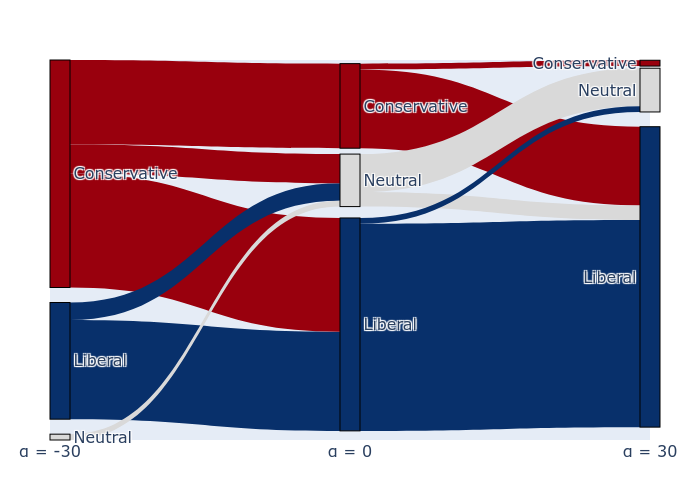
\includegraphics[width = 6in]{images/sankey_plot.png}
    \caption{Sankey diagram showing transitions in political bias labels across intervention strengths ($\alpha = -30 \rightarrow 0 \rightarrow 30$) at $k=32$ for LLaMA-2 7B. When the model is steered, it classifies identical texts relative to its new algorithmic frame.}
    \label{fig:sankey_bias}
    \end{center}
\end{figure}

As depicted in \autoref{fig:sankey_bias}, when LLaMA-2 is steered heavily toward the political left ($\alpha = -30$, interpreting the text through a mathematically enforced progressive lens), the majority of neutral or lightly partisan statements are consistently labeled as \textit{Conservative}. Conversely, steering the model toward the right ($\alpha = 30$) causes the exact same input batch to be substantially classified as \textit{Liberal}. 

\begin{table}[htbp]
    \centering
    \small
    \begin{tabular}{lccc}
        \toprule
        $k$ intervened & LLaMA-2 7B & LLaMA-3.1 8B & Qwen-2.5 7B \\
        \midrule
        8   & $-0.98$ & $\phantom{-}0.88$ & $-0.67$ \\
        16  & $\mathbf{-0.99}$ & $\phantom{-}0.43$ & $\phantom{-}0.35$ \\
        32  & $-0.97$ & $-0.55$ & $\mathbf{-0.99}$ \\
        64  & $-0.72$ & $\mathbf{\phantom{-}0.94}$ & $-0.91$ \\
        96  & $-0.85$ & $\phantom{-}0.83$ & $-0.81$ \\
        \bottomrule
    \end{tabular}
    \caption{Pearson correlation $r$ between intervention strength $\alpha$ and average bias classification labels across models. Negative correlations indicate that steering toward liberal ($\alpha<0$) causes the model to classify more statements as conservative, while positive correlations indicate the opposite.}
    \label{tab:pearson_bias}
\end{table}

The symmetric reversal indicates that steering the model along a latent ideological direction algorithmically shifts its political set-point. To quantify this relationship, I calculated the Pearson correlation coefficient $r$ between intervention strength $\alpha$ and the average parsed bias label. As shown in \autoref{tab:pearson_bias}, both LLaMA-2 7B and Qwen-2.5 7B follow this strong negative correlation pattern. The model evaluates third-party text relative to its own internal location on the manifold. In essence, the algorithmic equivalent of human confirmation bias functions reliably: as the model's geographic position is pushed left, the entire "center" of the political spectrum moves right relative to its coordinate system. 

Interestingly, LLaMA-3.1 exhibited reversed correlations compared to LLaMA-2 and Qwen. In LLaMA-3.1, steering the model liberal caused it to classify more statements as liberal. This indicates that LLaMA-3.1 collapsed the dimension of ideological representation and the dimension of bias-perception into identical semantic vectors during post-training fine-tuning, reflecting how different model families arrange identical data manifolds distinctly.

\subsection{Generalization to Voting Preference Prediction}

Simulating populations reliably requires models to faithfully reproduce behavioral choices. However, unlike the symmetry encountered in bias detection, manipulating behaviors for simulated ballot voting produced profound asymmetries and systemic distortions, mapped in \autoref{fig:vote_curve}. To avoid degenerate outputs during generation, I explicitly restricted interventions during the voting tasks to $\alpha \in \{-20,-10,0,10,20\}$ and $k \in \{16, 32, 64\}$, as extreme $\pm 30$ magnitudes frequently produced totally incoherent or stubbornly unreadable completions.

\begin{figure}[!htbp]
    \begin{center}
    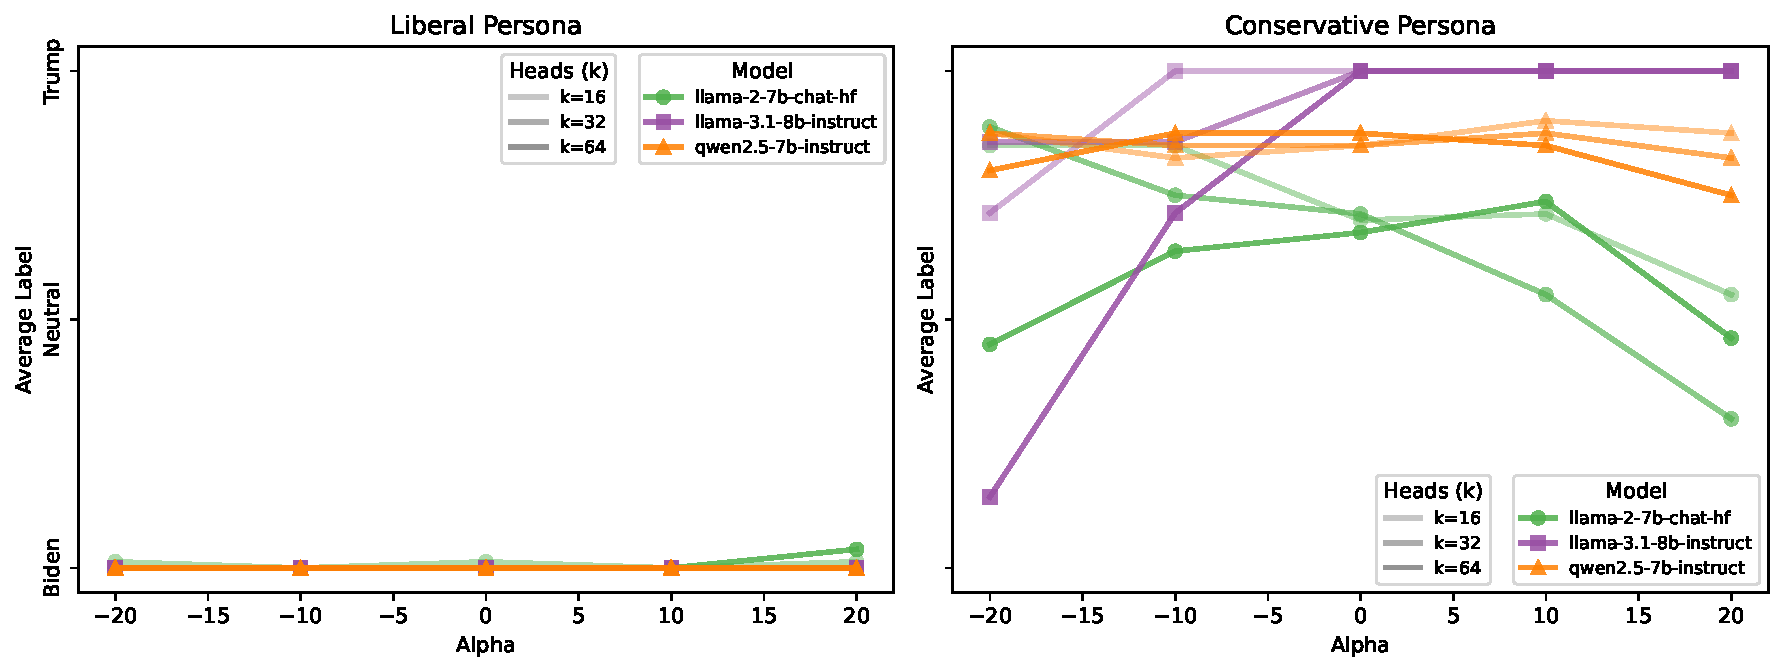
\includegraphics[width = 6in]{images/vote_intervention_models.pdf}
    \caption{Average predicted voting preference (Biden = -1, Trump = 1) across intervention strengths $\alpha$ for several models. Liberal personas resist all manipulation, while conservative prompts yield erratic model-dependent results.}
    \label{fig:vote_curve}
    \end{center}
\end{figure}

The \textbf{liberal persona} is highly resistant to steering across all three tested architectures. Irrespective of intervention magnitude $\alpha$ or the number of heads intervened $k$, the token outputs consistently favored Joe Biden. The baseline liberal prior is strongly embedded algorithmically. 

The \textbf{conservative persona} also displayed resistance, but the pattern was more erratic and model-dependent. LLaMA-3.1 8B and Qwen-2.5 7B exhibited a modest rightward shift in voting preference as $\alpha$ increased, but the effect was weak and inconsistent across $k$. In contrast, LLaMA-2 7B showed no clear directional shift; injecting conservative steering vectors into the forward pass paradoxically increased the likelihood of predicting a Biden vote over a Trump vote.

These results highlight two distinct phenomena: first, a broad \textit{unsteerability} in voting behavior, and second, a marked \textit{asymmetry} in the direction of that resistance. The unsteerability suggests that vote choice may not be directly controlled by the same latent partisan-ideological direction that governs bias detection and rewriting. Electoral preference may instead depend on additional representations, including candidate-specific valence, strategic heuristics, or task-level political knowledge, such that shifting a single ideological axis is insufficient to reliably reverse the behavioral output.

A second explanation for this same resistance is that the explicit partisan persona prompt anchors the model's internal state too strongly for the intervention to override. When the model is instructed to respond ``as a liberal'' or ``as a conservative,'' the persona priming itself may pre-activate and partially saturate the relevant region of the activation manifold before the intervention is applied. On this interpretation, the observed stability would not imply that ideology is irrelevant to voting, but rather that the prompt hardens the local representation and reduces the marginal effect of subsequent steering. This reading is consistent with recent findings by \citet{lampinenLinearRepresentationsLanguage2026}, who show that explicit user instructions can cause internal probes to activate on the instructed frame rather than solely on external facts.

The second phenomenon is the asymmetry of that resistance. Liberal personas are effectively always voting for Biden in this setup, whereas conservative personas are substantially less stable and, in some settings, become \textit{more} likely to vote for Biden rather than Trump. One plausible explanation is Reinforcement Learning from Human Feedback (RLHF) and related post-training alignment objectives. During alignment, models are rewarded for producing responses that appear helpful, harmless, cooperative, and socially acceptable. In the contemporary U.S. political context, those ratable traits may be more statistically aligned with mainstream liberal or center-left linguistic norms than with strongly conservative political expression. If so, the model may acquire a default behavioral prior that is "friendly" in a manner that is not politically neutral \citep{potterHiddenPersuadersLLMs2024}. Under this interpretation, the persistent Biden preference is not simply a statement about partisan ideology, but about how alignment training reshapes politically charged response space. Pushing the model further into a conservative region may therefore activate safety or helpfulness corrections that redirect the output toward a more institutionally approved, Biden-favoring response. This cautionary pattern serves as a warning against naively treating aligned LLMs as transparent simulators of electoral preference in CSS, and also to attempts to perform such simulations with steered models without first validating the causal effects of that steering on voting behavior.

\subsection{Generalization to Bias Neutralization via Rewriting}

I instructed models to neutralize ideologically charged statements under varied steering vectors. This evaluates whether latent ideology subtly modulates stylistic and lexical semantic choices beyond raw classification. 

\begin{table}[!htbp]
\centering
\small
\begin{tabular}{clp{10cm}}
\toprule
\textbf{$\alpha$} & \textbf{Steer} & \textbf{Output Excerpt} \\
\midrule
$ -$ & Original &
``As we navigate... it is essential to respect individuals' privacy while also ensuring that all students feel safe...'' \\
\addlinespace[0.5em]
$-30$ & Liberal &
``...recognize the importance of respecting individuals' privacy... while also addressing the ongoing struggle for justice and equality in the face of systemic oppression and discrimination.'' \\
\addlinespace[0.5em]
$0$ & Neutral &
``...strike a balance between respecting individuals' privacy and creating an inclusive environment...'' \\
\addlinespace[0.5em]
$30$ & Conservative &
``...consider the privacy of individuals... specific actions and preferences of individuals should be taken into account...'' (incoherent continuation follows) \\
\bottomrule
\end{tabular}
\caption{Impact of latent ideology on neutrality rewriting. Heavy steering overrides the core instruction prompt, forcing the adoption of specific partisan vocabularies.}
\label{tab:neutralization_outputs}
\end{table}

The baseline unsteered model ($\alpha = 0$) performs the task effectively, removing the partisan phrasing and providing balanced academic rhetoric. However, the $\alpha = -30$ injection substantially alters the instruction prompt to remain "neutral." As seen in Table \ref{tab:neutralization_outputs}, the leftward vector leads to the adoption of modern progressive academic vocabulary ("systemic oppression", "ongoing struggle for justice"). The model conflates strong progressive orientation with its natural baseline generative vocabulary for sociology. 

\begin{figure}[!htbp]
    \begin{center}
    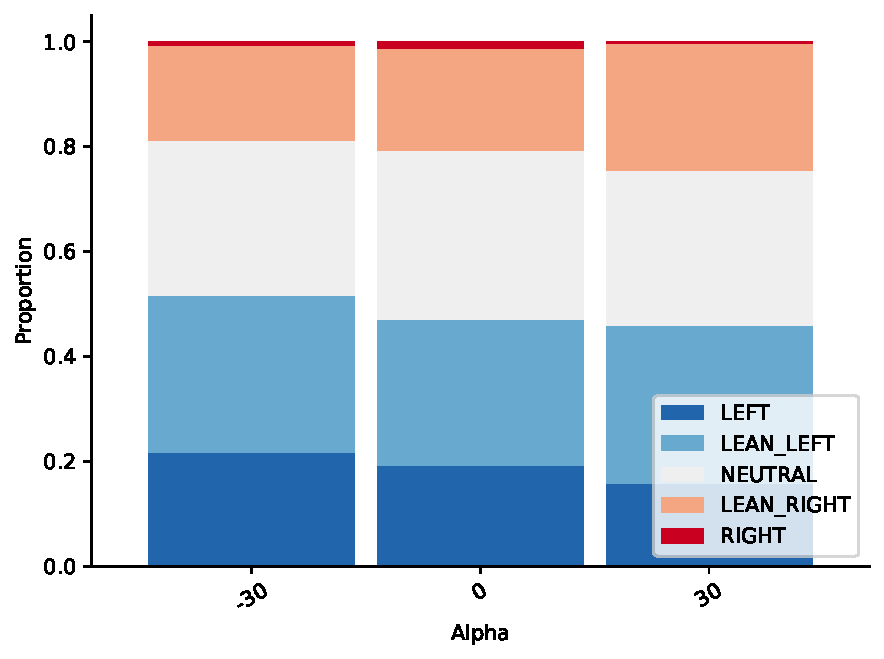
\includegraphics[width = 4.6in]{images/rewrite_intervention_plot.pdf}
    \caption{GPT-5 classification of the generated rewrites. High magnitude interventions destroy neutrality, polarizing the rewritten text along partisan lines.}
    \label{fig:rewrite_plot}
    \end{center}
\end{figure}

Conversely, the $\alpha = 30$ high-magnitude conservative injection highlights "individual actions" but swiftly fragments into grammatical incoherence, mirroring the RLHF constraint conflict observed in the voting simulations. These findings demonstrate that latent linear interventions strongly influence abstract generative style and lexicon, often decoupling the generated text from the explicit neutrality instruction of the system prompt.


\section{Results: Ideological Generalization in Vision Models}
\label{resultsvision}

Having established a text-domain ideological direction, I next examine whether related structure is observable in vision-language representations.

\subsection{Validating the Generalization Across Text and Vision}

Before applying the text-derived politician direction to open-world imagery, I first evaluate it on two labeled visual corpora: official congressional portraits and partisan Twitter images. This validation step reduces the risk of over-interpreting heatmap patterns and provides an empirical basis for cross-modal claims. If the text-derived direction distinguishes politicians in both controlled portraits and noisier real-world posts, it is more plausible to treat it as a shared text-vision ideological axis.

I applied the DW-NOMINATE text probe to the sequence activations of Qwen3-VL image tokens.

\begin{figure}[H]
    \centering
    \begin{subfigure}{0.35\textwidth}
        \includegraphics[width=\linewidth]{../../vision-political-llm/peter/blogs/images/B001281.jpg}
    \end{subfigure}
    \hspace{0.5cm} % Adjust this value to bring them closer or further apart
    \begin{subfigure}{0.35\textwidth}
        \includegraphics[width=\linewidth]{../../vision-political-llm/peter/blogs/images/B001282.jpg}
    \end{subfigure}
    \caption{Example congressional portraits from the 116th Congress, shown for qualitative context (Democrat at left; Republican at right).}
    \label{fig:portrait_examples}
\end{figure}

On the 550 official portraits from the 116th Congress, mean probe scores were generally higher for Republican faces and lower for Democratic faces. Higher-magnitude token scores were often concentrated around facial regions, and the the score positively correlates with the politician's DW-NOMINATE position ($r = 0.54$, see \autoref{fig:portrait_correlation_text_probe}). One plausible explanation is that the model can recognize at least some of these public figures directly, especially because congressional names were used in the text-domain probe construction. If so, the portrait result is still substantively informative: it indicates that visual recognition of politicians is mapped onto the same direction that, in the text experiments above, behaved as an ideological rather than merely identity-based dimension. These results are therefore consistent with the interpretation that at least part of the text-domain ideological direction is reflected in visual token representations under controlled photographic conditions.

\begin{figure}[H]
    \centering
    
\includegraphics[width=0.95\textwidth]{../../vision-political-llm/peter/blogs/images/congress_images_correlation_politician.png}
    \caption{Portrait-level validation using the text-derived ideological direction. The figure plots per-portrait mean image-token score against DW-NOMINATE score, showing a positive correlation across members of Congress ($r = 0.54$).}
    \label{fig:portrait_correlation_text_probe}
\end{figure}

\begin{figure}[H]
    \centering
    \includegraphics[width=0.85\textwidth]{../../vision-political-llm/peter/blogs/images/coloring_portraits_textual_probe.png}
    \caption{Token-level ideology heatmapping on the congressional portrait validation set using the text-trained politician direction. The top-left panel shows the mean token score map for Democratic portraits, and the top-right panel shows the corresponding mean map for Republican portraits. The bottom-left panel reports the party difference map (Republican minus Democratic), with the largest contrast concentrated near eye level. The bottom-right panel summarizes portrait-level mean scores by party, showing a distributional separation between Democratic and Republican portraits.}
    \label{fig:portrait_validation}
\end{figure}

I then evaluate the same direction on the Twitter validation set containing 1367 images posted by congressional Democrats and Republicans. This set is substantially noisier than portraits, including rallies, crowds, graphics, memes, and informal photographs. After averaging token scores within each image, partisan differences remain observable at the distributional level, and the member-level average image score correlates with the posting politician's DW-NOMINATE score ($r = 0.58$). It remains possible that some tweet-image pairings, or their surrounding discourse, were seen during pretraining. However, that possibility does not weaken the central interpretive point of this section. In light of the previous text experiments, which showed that the politician direction also functions as an ideological direction across textual tasks, the Twitter result suggests that the model jointly associates politicians, party labels, ideological position, and their textual and visual representations along a common internal axis. While this evidence remains correlational, it suggests that the text-derived direction is not limited to studio-like headshots and remains detectable in heterogeneous political imagery.

\begin{figure}[H]
    \centering
    
\includegraphics[width=0.8\textwidth]{../../vision-political-llm/peter/blogs/images/twitter_example_rep.png}
    \caption{Example partisan Twitter image posted by a Republican member of Congress with the text-derived ideology heatmap overlaid.}
    \label{fig:twitter_example}
\end{figure}

\begin{figure}[H]
    \centering
    
\includegraphics[width=0.85\textwidth]{../../vision-political-llm/peter/blogs/images/twitter_member_level_dw.png}
    \caption{Member-level correlation between average Twitter-image probe score and the posting politician's DW-NOMINATE score ($r = 0.58$). The observed association is consistent with cross-modal generalization of the text-derived direction.}
    \label{fig:twitter_validation}
\end{figure}

Taken together, the portrait and Twitter validations provide preliminary support for using the text-trained politician direction as a discovery tool in vision. The portrait setting shows that recognized political individuals can be located on this axis from visual input alone, while the Twitter setting indicates that the same axis remains recoverable in more naturalistic and semantically cluttered imagery. Combined with the earlier textual results establishing that this politician direction also carries ideological content, these validations support the narrower claim advanced here: within the model, politician identity, party affiliation, ideological position, and their textual and visual manifestations appear to be at least partially organized along a shared representational direction. Accordingly, in the remainder of this section I apply it to unlabeled images as an exploratory instrument for identifying visual motifs that align with the same liberal-conservative axis.

\subsection{Discovering Political Iconography in the Wild}

To move beyond explicitly political photography, I apply the text ideology probe to a large corpus of 25,000 generic images from Unsplash.

Given the prior portrait and Twitter validations, I treat the Unsplash analysis as a zero-shot exploratory exercise rather than a test of predictive accuracy. The purpose is not to claim that these generic images possess ground-truth ideological labels, but to examine whether a direction validated on explicitly political imagery also surfaces regularities in images that are not overtly political at first sight.

Substantively, this exploratory step asks whether the model extends political organization beyond formal political objects and actors into broader cultural iconography. If so, that would suggest that seemingly apolitical visual content is nevertheless embedded within learned political associations: not because every such image is inherently political, but because the model has absorbed recurrent internet correlations that connect certain aesthetics, places, demographics, and objects to ideological categories. In that sense, the Unsplash exercise is intended as a discovery procedure for latent politicization in the wild.

Consistent with that framing, the heatmaps suggest that the VLM organizes some recurring aesthetic signifiers of political affiliation along the same axis.
\begin{itemize}
    \item \textbf{Liberal Vector Triggers}: The model associates dense urban environments, large crowds spanning diverse demographics, environmental protests, LGBTQ+ iconography, public transport, and progressive bohemian fashion heuristics strongly with the liberal text vector.
    \item \textbf{Conservative Vector Triggers}: In contrast, the VLM associates wide-open rural landscapes (e.g., herds of cattle), cowboys, gas stations, and traditional Americana settings with the conservative text vector.
\end{itemize}

\begin{figure}[H]
    \centering
    \begin{subfigure}{0.32\textwidth}
        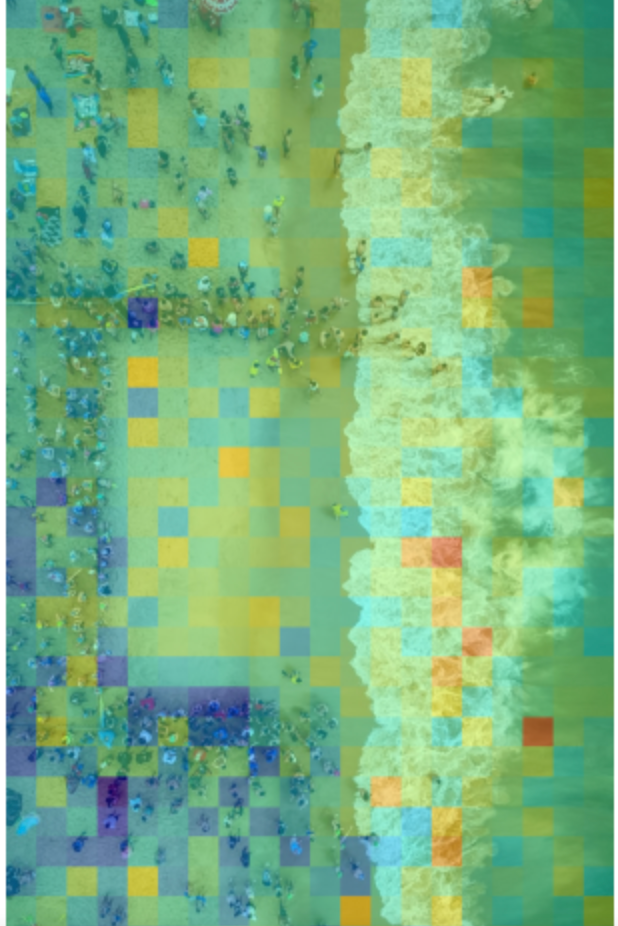
\includegraphics[width=\linewidth]{images/heatmap_left_1.png}
    \end{subfigure}
    \hfill
    \begin{subfigure}{0.32\textwidth}
        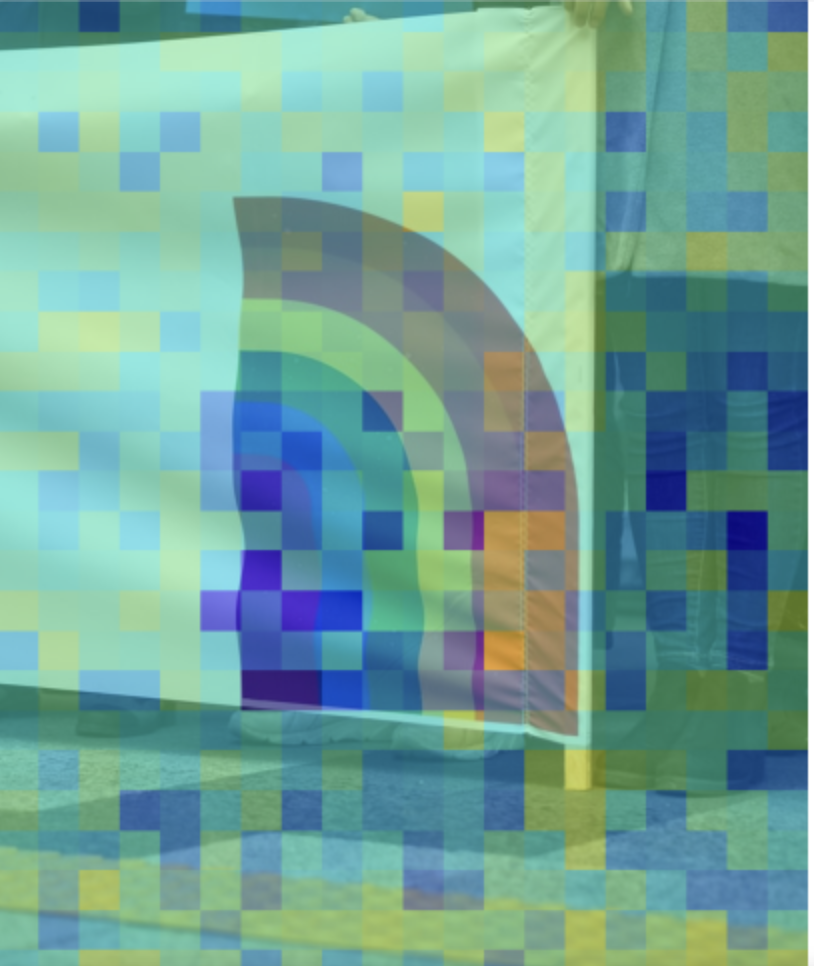
\includegraphics[width=\linewidth]{images/heatmap_left_3.png}
    \end{subfigure}
    \hfill
    \begin{subfigure}{0.32\textwidth}
        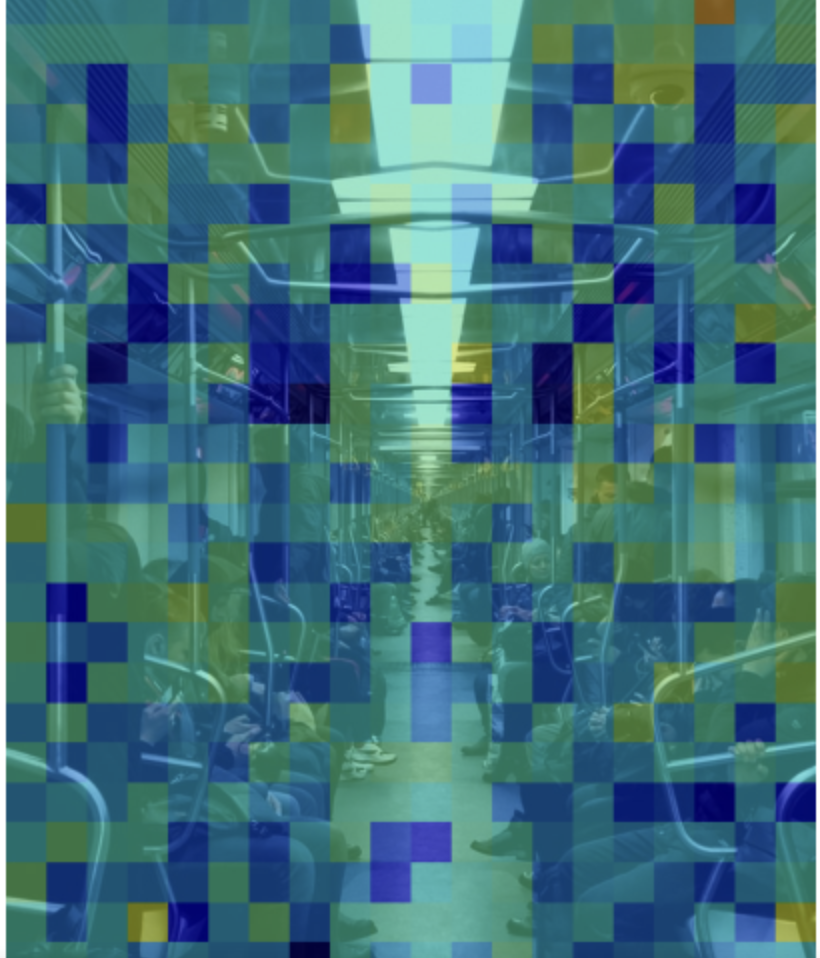
\includegraphics[width=\linewidth]{images/heatmap_left_4.png}
    \end{subfigure}
    \caption{Zero-shot visual triggers for the mathematical ``Liberal'' textual vector on unstructured Unsplash imagery. The architecture implicitly correlates left-wing ideology with diverse demographics, Pride aesthetics, and public transit structures.}
    \label{fig:unsplash_liberal}
\end{figure}

\begin{figure}[H]
    \centering
    \begin{subfigure}{0.48\textwidth}
        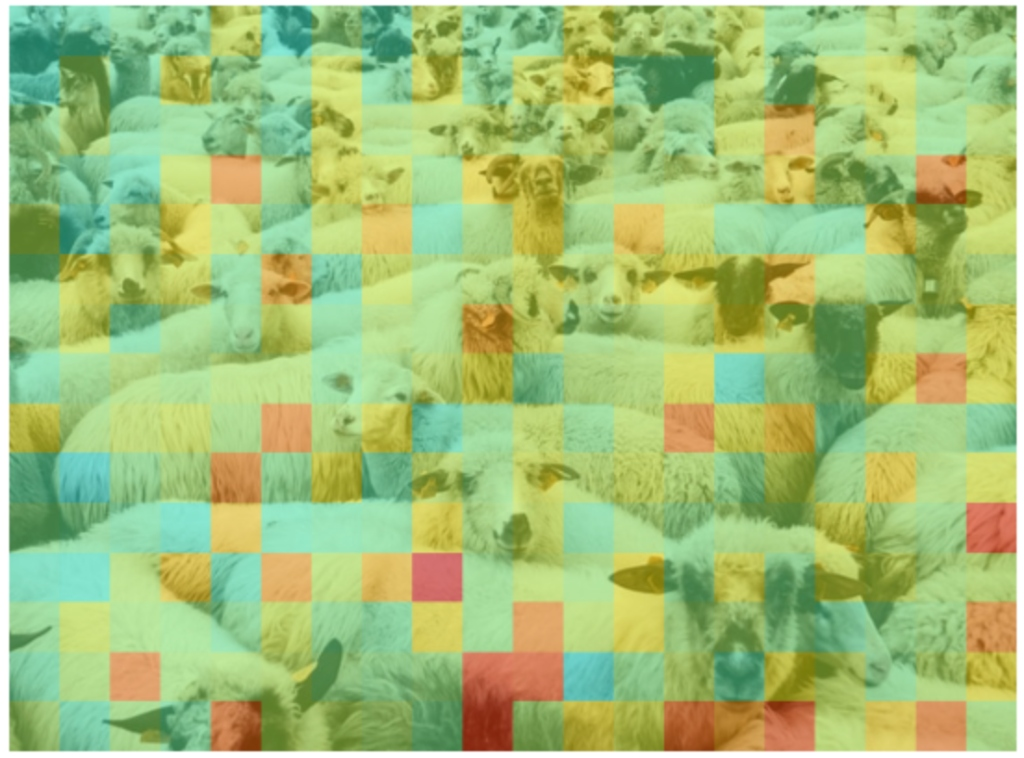
\includegraphics[width=\linewidth]{images/heatmap_right_1.jpg}
    \end{subfigure}
    \hfill
    \begin{subfigure}{0.48\textwidth}
        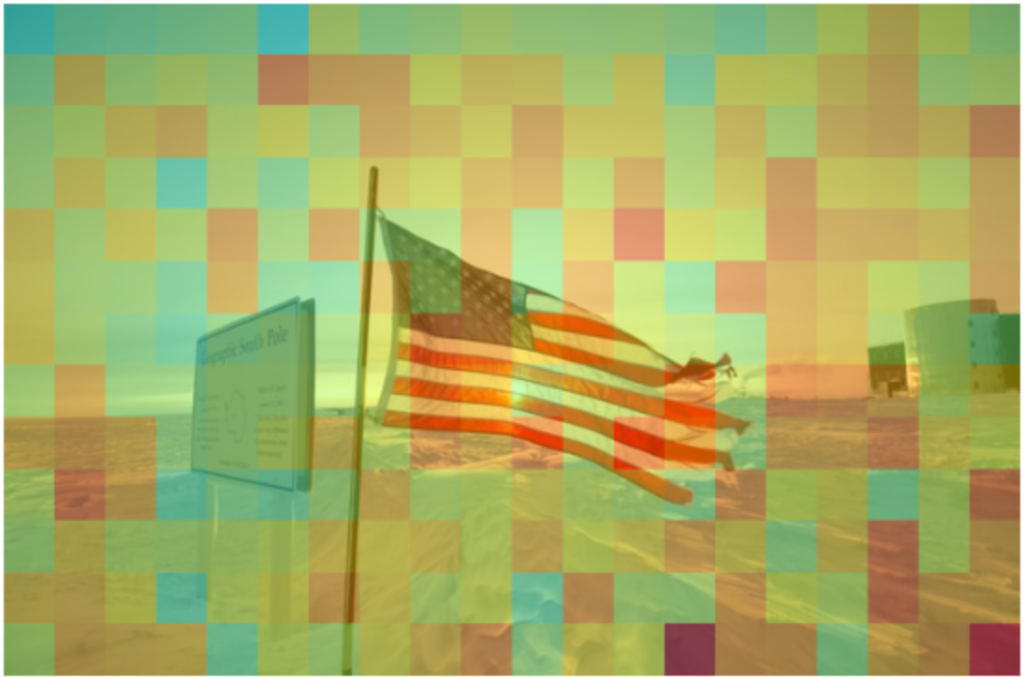
\includegraphics[width=\linewidth]{images/heatmap_right_2.png}
    \end{subfigure}
    \vspace{0.2cm}

    \begin{subfigure}{0.48\textwidth}
        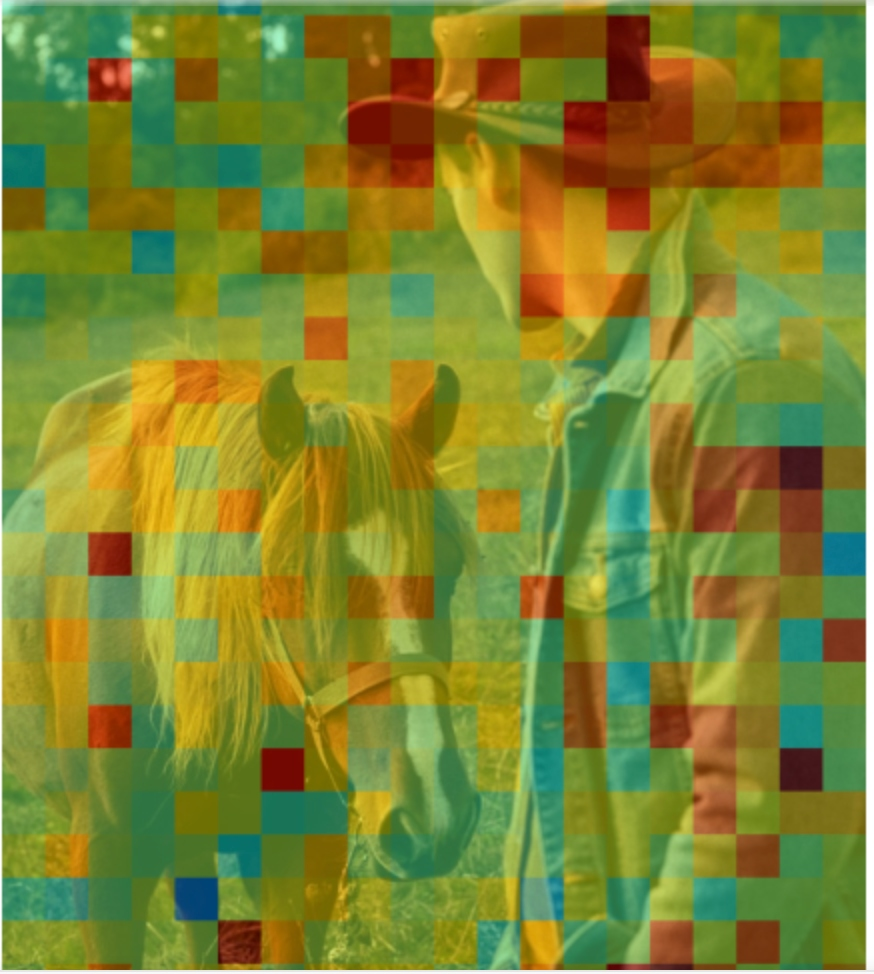
\includegraphics[width=\linewidth]{images/heatmap_right_3.jpg}
    \end{subfigure}
    \hfill
    \begin{subfigure}{0.48\textwidth}
        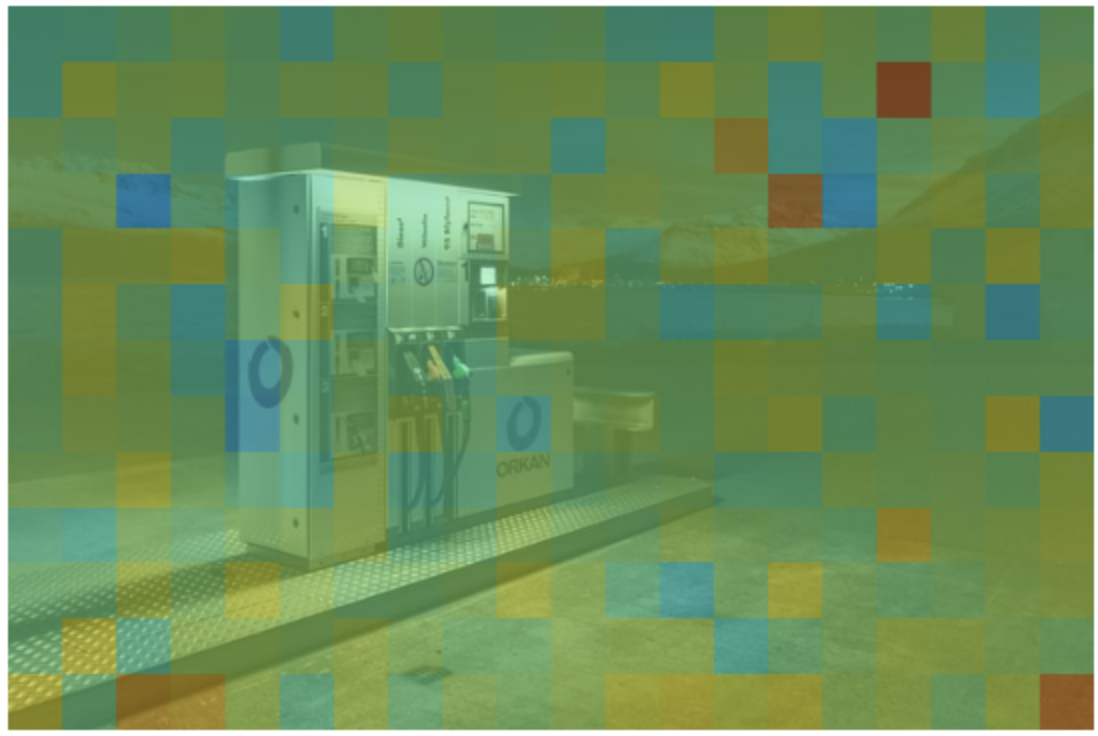
\includegraphics[width=\linewidth]{images/heatmap_right_4.png}
    \end{subfigure}
    \caption{Zero-shot visual triggers for the ``Conservative'' vector. The latent space intrinsically binds right-wing political identity with rural Americana, cowboys, heavy infrastructure, and agrarian landscapes.}
    \label{fig:unsplash_conservative}
\end{figure}

These patterns are consistent with the interpretation that the foundational model has learned culturally familiar associations from paired internet imagery, including a divide between liberal-coded dense urban scenes and conservative-coded rural or industrial scenes. At the same time, this evidence should be treated as qualitative and hypothesis-generating rather than definitive. The present analysis identifies suggestive motifs, but it does not yet provide a comprehensive extraction of the full set of visual associations carried by the model, especially for images whose political content is indirect, ambiguous, or not political on first inspection. Future work should therefore develop more systematic procedures for large-scale association extraction and validation in order to map everyday iconography that is the most consistently organized along these latent political dimensions.

\subsection{Steering Aesthetic Generation in Unified Language Models}

A clear demonstration of the causal entwinement of text and vision modalities is my capacity to steer generated imagery utilizing text-vector arithmetic inside the Unified Language Model Janus-Pro.

By directly manipulating the forward sequence generation parameters utilizing my ITI text methodology—replacing natural attention activations with ideological additions—I systematically altered the visual scene generated by the generic prompt: \textit{"A politician"}.

\begin{figure}[!htbp]
    \begin{center}
    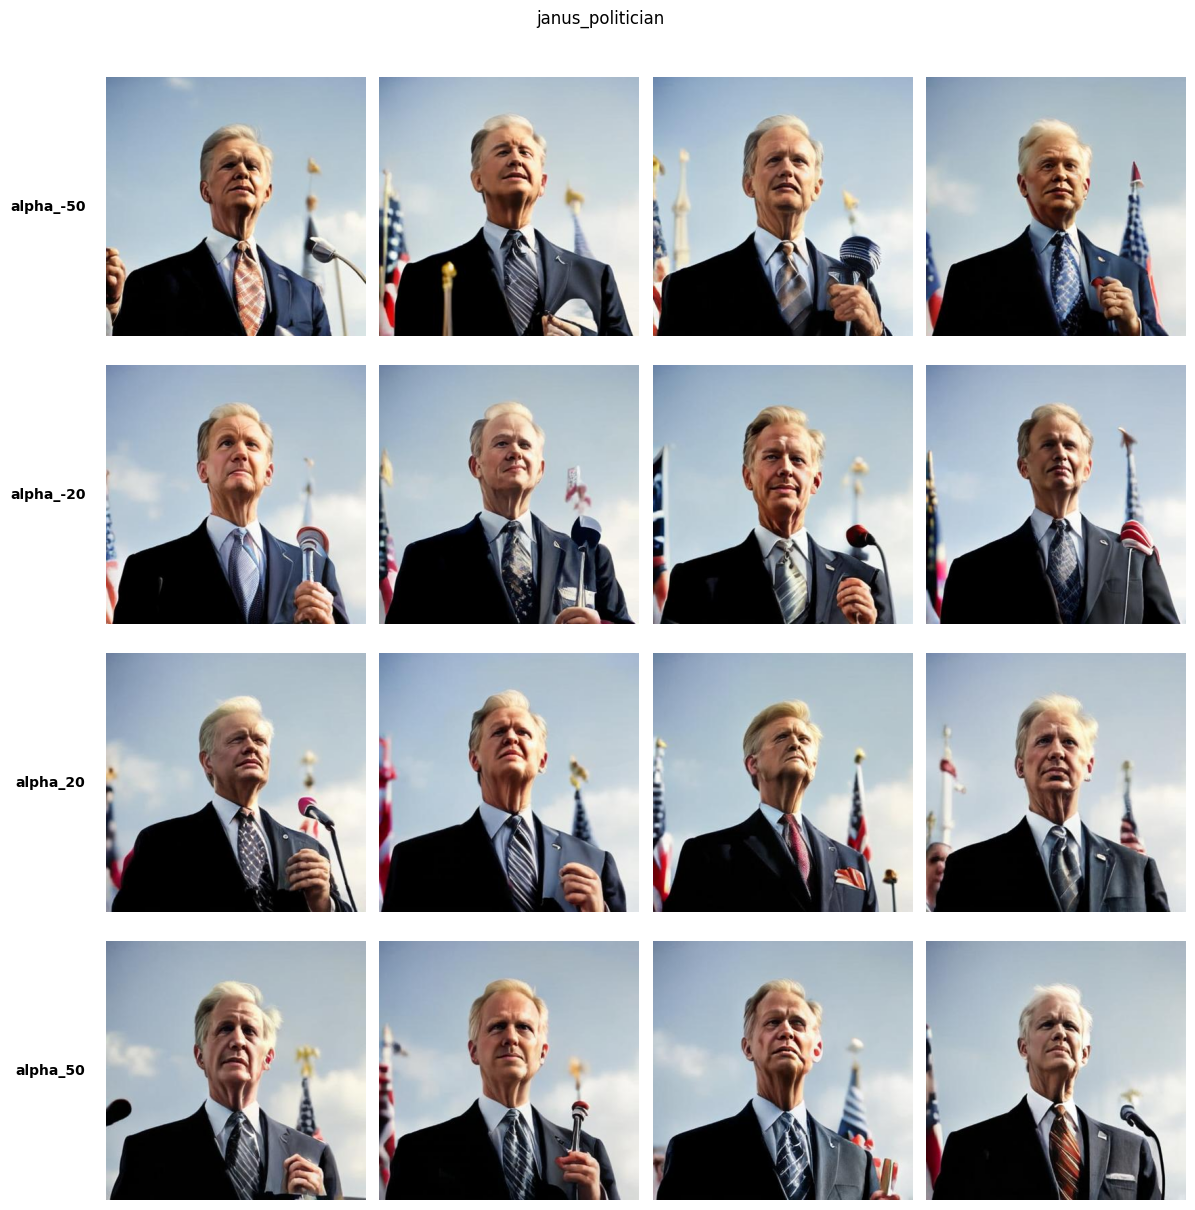
\includegraphics[width = 5in]{images/janus_politician.png}
    \caption{Generational output for the minimal prompt "A politician", steered algorithmically across the liberal-conservative axis. Textual linear math strongly influences the visual representation.}
    \label{fig:janus_politician}
    \end{center}
\end{figure}

As shown in \autoref{fig:janus_politician}, while the overarching structural staging of the image remains relatively constant, scaling $\alpha$ backward and forward triggers subtle but consistent contextual shifts. Notably, leftward progressive steering introduces significantly softer, more relaxed facial expressions. Conversely, rightward conservative steering enforces rigid posture and more severe expressions, likely driven by the text-based DW-NOMINATE steering vectors.

To test if these textual ideology vectors could override the rigid latent embeddings of a highly polarized, specific real-world figure, \autoref{fig:janus_hillary} illustrates the ULM generation for \textit{"Hillary Clinton"}.

\begin{figure}[!htbp]
    \begin{center}
    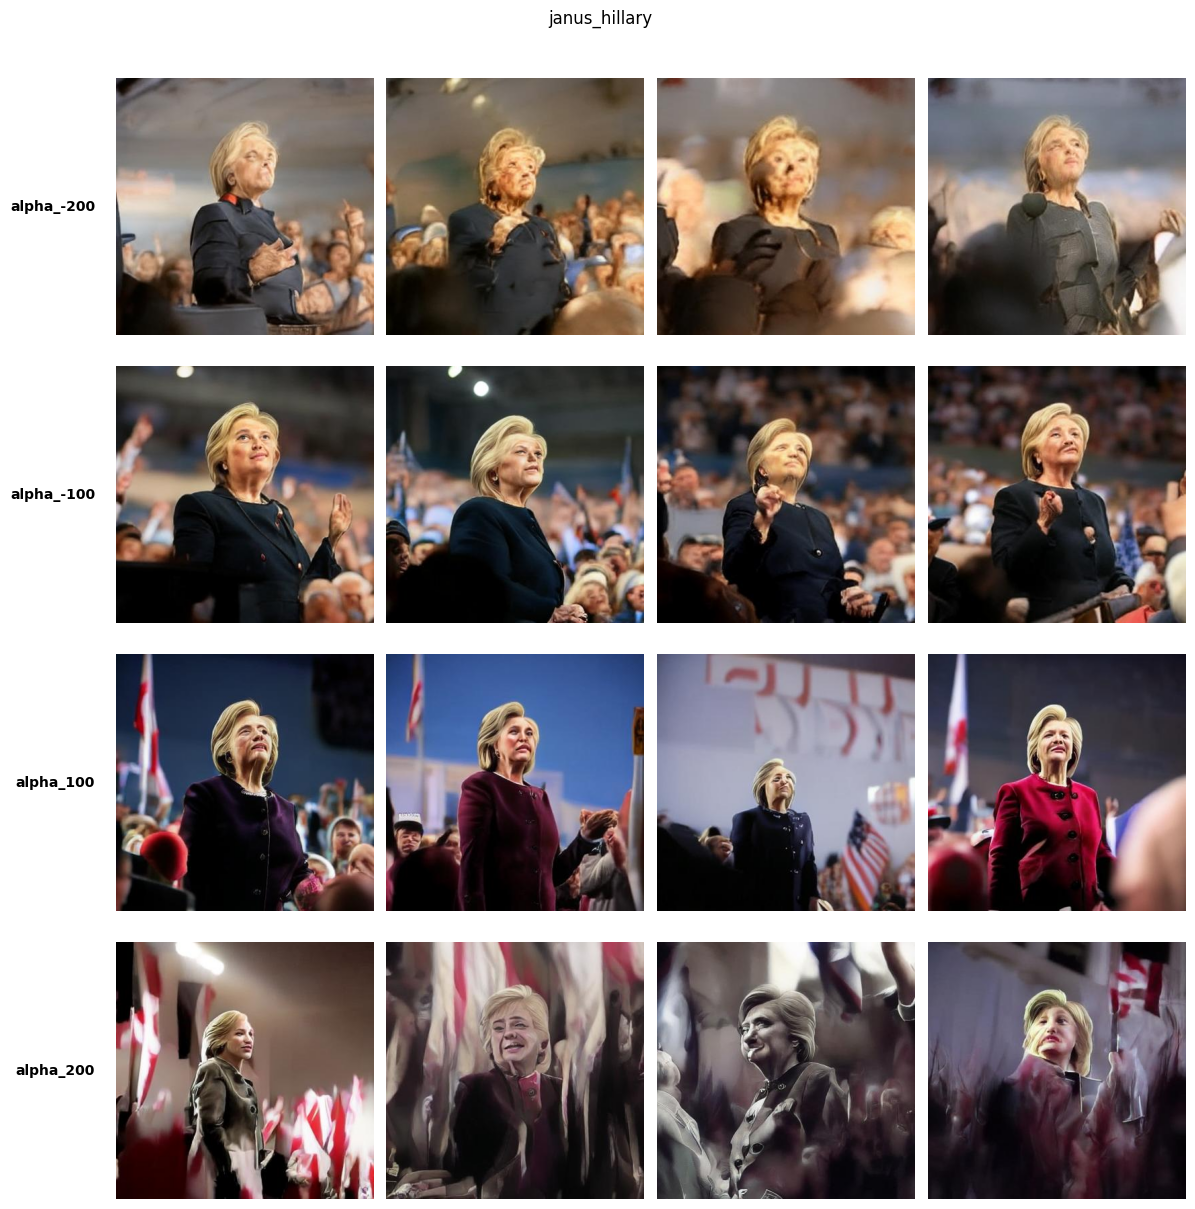
\includegraphics[width = 5in]{images/janus_hillary.png}
    \caption{Steering applied to a specific, highly polarized real-world figure. Ideological steering alters the generated aesthetic and perceived narrative without explicitly prompting the model for ideological changes.}
    \label{fig:janus_hillary}
    \end{center}
\end{figure}

The ideological steering effectively bypassed the model's hardened representation of the specific identity, imposing aggressive new visual narratives. Pushing Hillary Clinton "further left" portrays her intensely illuminated by bright spotlights, closely surrounded by crowds of comrades, and dressed in a high-collared Zhongshan suit. Conversely, pushing her heavily "right" structurally darkens the visual color grading, outfits her in a heavy black leather jacket, and imposes a severe, authoritarian aesthetic absent in the baseline ($\alpha=100$ and $\alpha=-100$) generation.

These results suggest that the text-based ideological vectors are not only entangled with the visual generation pathway but can also override specific identity representations to impose new visual narratives. This provides compelling evidence for a shared latent geometry across modalities, where abstract political concepts derived from text can directly influence the visual heuristics of generated imagery, which has profound implications for understanding how biased representations might propagate across different content types in unified models under politically charged generation tasks.

\section{Discussion}
\label{discussion}

\subsection{Ideological Geometry: Intertwined Dimensions}
The empirical findings presented in this research build upon recent literature investigating how foundational architectures natively represent political ideology \parencite{kimLinearRepresentationsPolitical2025, gurneeLanguageModelsRepresent2023}. By structuring an Inference-Time Intervention (ITI) probe using the DW-NOMINATE liberal-conservative spatial continuum \parencite{carrollMeasuringBiasUncertainty2009}, the results suggest that these latent representations are closely related to broader behavioral dimensions. Rather than merely adopting a persona, manipulating the model's internal activations yielded predictable, systematic shifts in downstream tasks such as political bias detection. When steered, LLaMA-2 recalibrated its categorization of neutral text based on the newly imposed ideological vector, indicating that the representation correlates strongly with the model's internal evaluation logic.

Importantly, the strength of this generalization claim partly follows from the very limitation that might initially seem to weaken it. DW-NOMINATE is deeply entangled with partisan sorting, and my probing procedure begins with politician names. On its face, this raises the possibility that the recovered direction is a hardened politician-party recognition axis rather than an ideological representation in any richer sense. Yet the empirical results extend well beyond the original name-conditioned setting. The same direction influences ideological evaluations of statements, shifts bias-detection outputs, alters the rhetoric of neutrality rewriting, tracks partisan styles in congressional Twitter imagery, and partially organizes portrait representations. This broader transfer suggests that, within the models studied here, politician identity, party label, ideological orientation, and downstream political judgements are not cleanly separable. If anything, the fact that a politician-anchored probe travels so effectively across these heterogeneous tasks strengthens the claim that the models have fused these attributes into a common political geometry.

Furthermore, the generative rewrite task demonstrated that these ideological dimensions are intertwined with specific structural rhetorics. Steering the model leftward not only shifted the policy stance of the generated text but simultaneously introduced specific academic sociological terminology (e.g., "systemic oppression"). This behavior suggests that the DW-NOMINATE axis cannot be easily isolated; it appears entangled with stylometrics and the model's learned vocabulary for specific worldviews. Additionally, the behavioral asymmetries observed during the voting preference predictions—where conservative steering frequently collapsed into progressive responses—highlight potential correlations between political representations and the safety guardrails established during Reinforcement Learning from Human Feedback (RLHF) \parencite{pmlr-v202-santurkar23a, guptaBiasRunsDeep2023}. This entanglement complicates the use of foundation models as neutral demographic proxies, as safety alignment protocols may heavily modulate polarized ideological representations.

\subsection{Generalized Ideological Dimension Across Modalities}
By extending this latent analysis into Vision-Language Models (VLMs) and Unified Language Models (ULMs), this research provides a potential framework for cross-modal ideological mapping. In bridging text-based DW-NOMINATE vectors to the image patching mechanics of Qwen3-VL, the textual probe serves as an effective proxy to systematically analyze the visual symbols the model associates with the political divide. The resultant heatmaps suggest that the model organizes visual aesthetics—such as rural landscapes and agricultural settings versus diverse urban crowds and public transit—along a continuously shared representational dimension.

The generative results derived from Janus-Pro offer further experimental support for this cross-modal relationship. Demonstrating that a mathematical formulation extracted entirely from textual roll-call data can systematically influence the lighting, demographic compositions, and clothing selections (e.g., contrasting formal attire with relaxed styling) of generated images reveals a notable association between text-based ideology and visual heuristics. These findings suggest that the foundational layers likely utilize paired multimodal internet training data to correlate legislative speech patterns with specific cultural visualizations. The application of textual probes in this manner provides researchers with a novel proxy metric to interpret how emerging unified architectures map abstract sociopolitical concepts across diverse visual outputs.

\subsection{Strengths and Limitations}
A primary methodological strength of this research lies in its causal framing. By utilizing ridge regression for linear probe optimization and evaluating the models through programmatic Inference-Time Interventions, the findings are largely isolated from the superficial confounding variables typically associated with prompt engineering. Mathematically manipulating the continuous activation sequence provides a more reliable metric for assessing the structural role of the localized ideology compared to merely observing a model mimic a prompted conversational style. Moreover, executing these text-derived interventions natively on the visual generation pathway of Janus-Pro introduces a promising methodological technique for probing multi-modal integration.

However, several limitations must be carefully acknowledged. First, the methodology relies exclusively on a one-dimensional (liberal-conservative) proxy of ideology derived from the elite voting records of the U.S. 116th Congress. As established by \citet{mccartyDefenseDWNOMINATE2016}, modern political ideology is increasingly multidimensional, influenced by orthogonal axes such as populism, libertarianism, and religious traditionalism, which are not captured by this single spatial model. Second, the linear ITI structure assumes that political beliefs are linearly separable within the high-dimensional latent space. Subsequent non-linear probing architectures may reveal that complex sociopolitical concepts form complicated, curved manifolds that resist simple scalar interventions. Finally, while the cross-modal ULM results demonstrate a clear semantic crossover, the exact physical circuitry explaining how the visual encoder mathematically translates pixel clusters into the identical vector space as legislative text remains unmapped. Future research requires more granular, layer-by-layer mechanistic interpretability to fully trace the mechanics of this modality transition.

An additional limitation is that the present probe is anchored to politician-centered supervision. Because DW-NOMINATE and party identity are tightly coupled in contemporary U.S. politics, the recovered direction likely mixes ideological content with elite recognition and partisan categorization. That mixture is itself substantively revealing for how models organize political information, but it also means the current design cannot fully separate ideology from politician-centered cues. A natural next step would be to construct alternative probes from manifesto or platform text and test whether those directions recover the same downstream structure. If a manifesto or political opinion derived direction could still classify the party affiliation of politician names, speeches, or portraits, that would provide stronger evidence that the shared latent dimension is not merely a byproduct of politician recognition, but a more general political axis internal to the model, and the underlying human data generation process.

\section{Conclusion}
\label{conclusion}

This research investigated whether latent representations of political ideology in open-weight foundation models function merely as passive correlates entirely dependent on prompts or as active structural pathways governing downstream behaviors. By applying Inference-Time Interventions aligned to the DW-NOMINATE axis, the findings indicate that these architectures consistently abstract political discourse into functional representations. Steering these internal values yielded predictable shifts in the models' fundamental reasoning logic, steadily recalibrating their baseline approaches to political bias detection and modifying their vocabulary selection during text generation tasks.

Furthermore, extending this methodology to Vision-Language architectures (Qwen3-VL) and Unified Language Models (Janus-Pro) provided evidence for cross-modal ideological mapping. Treating the localized textual dimension as a proxy to analyze visual heuristics revealed that the models systematically associate the abstract political divide with contrasting aesthetics—for instance, correlating rural environments and structured attire with conservatism. The capacity to influence the staging of generated multimedia by manipulating an isolated linear text vector suggests that foundation models may organize semantic concepts along an embedded, modality-agnostic manifold.

The behavioral constraints observed during these interventions highlight significant implications for Computational Social Science researchers. The discovery that aggressive conservative steering can paradoxically induce progressive voting preferences suggests that safety alignment protocols, such as RLHF, may structurally warp the geometry of highly polarizing views. Consequently, researchers executing social simulations using AI agents must exercise careful methodological caution; treating foundation models as straightforward proxies for diverse human demographics risks inadvertently mapping the artificial boundaries of safety guardrails rather than authentic sociological variations.

\vfill
{\normalsize \section*{Data and Code Availability Statement}}
Replication code for the inference-time interventions and cross-modal generations is publicly available on GitHub at \href{https://github.com/DotIN13/linear-political-llm/tree/dev}{https://github.com/DotIN13/linear-political-llm/tree/dev}. The dataset of simulated political policy statements utilized for bias and neutralization evaluations can be accessed via Hugging Face at \href{https://huggingface.co/datasets/DotIN13/political-statements}{DotIN13/political-statements}. The Unsplash 25k imagery dataset leveraged to evaluate baseline cultural aesthetics is hosted at \href{https://huggingface.co/datasets/jamescalam/unsplash-25k-photos}{jamescalam/unsplash-25k-photos}.

\newpage
\setlength{\bibparsep}{0pt}
\section*{References}
\label{references}
\printbibliography[heading=none]

\end{document}
